
\begin{frame}{\citetitle{ProyectoLSM_2022}$^*$  (1)}
\begin{columns}
\begin{column}{0.6\textwidth}
	\begin{itemize}
		\item Se propone una aplicación móvil que reconozca el lenguaje de señas mexicano (LSM)
        \item El equipo capturó videos de los diferentes gestos a clasificar (palabras comunes y letras del alfabeto)
        \item Se utilizó la libreria MediaPipe para la obtención de los marcadores de manos, torso y cabeza
        \item Se entrenó una Red Neuronal Convolucional
	\end{itemize}
\end{column}
\begin{column}{0.4\textwidth}  
\begin{center}
     \begin{tabular}{cc}

         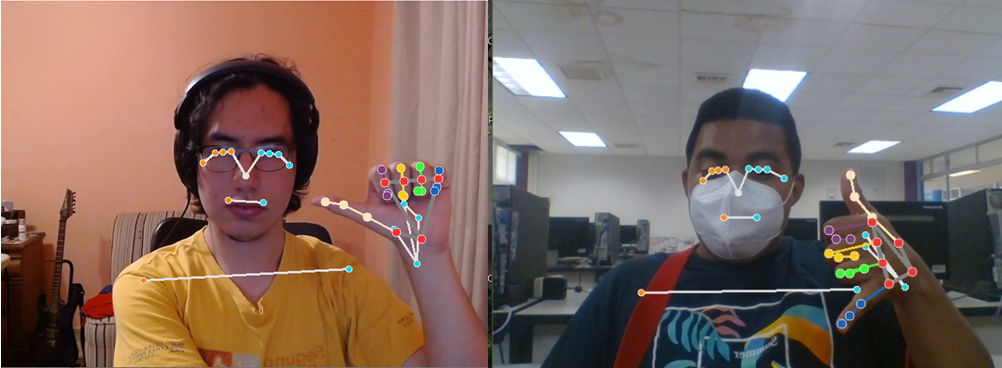
\includegraphics[width=0.98\textwidth]{2022_AplicacionLSM/figs/Diapositiva1.PNG}\\         
      \end{tabular}
\end{center}
\end{column} 
\end{columns} 
\footfullcite*{ProyectoLSM_2022}
\end{frame}


\begin{frame}{\citetitle{ProyectoLSM_2022} (2)}
\begin{columns}
\begin{column}{0.6\textwidth}
Librerías utilizadas:
\begin{itemize}
        \item Tensorflow (PC) y Tensorflow-lite (Smartphone)
		\item MediPipe
	\end{itemize}
Para cada video:
\begin{itemize}
        \item Se normaliza la duración del video a una duración estándard
		\item Se entraen ubicaciones de los marcadores y se estiman angulos
		\item Se anexa al dataset para su posterior entrenamiento
	\end{itemize}
\end{column}
\begin{column}{0.4\textwidth}  
\begin{center}
     \begin{tabular}{c}
         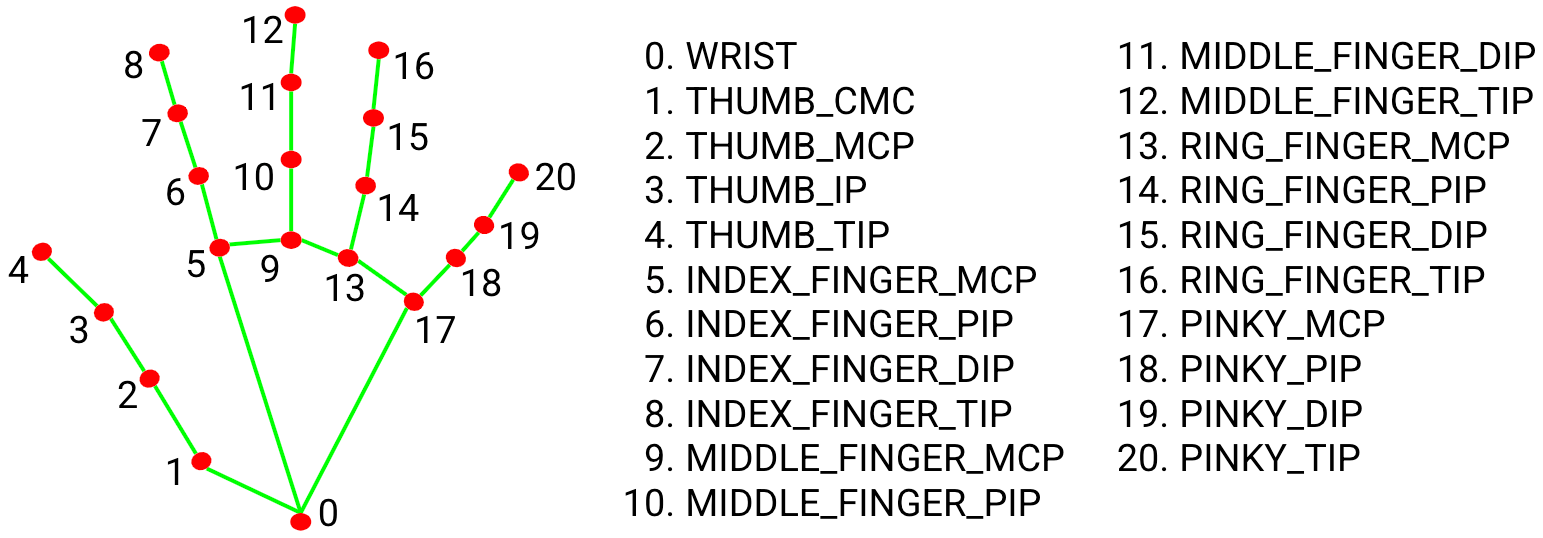
\includegraphics[width=0.98\textwidth]{2022_AplicacionLSM/figs/hand_landmarks.png}\\
          \end{tabular}
\end{center}
\end{column} 
\end{columns} 
\end{frame}

\begin{frame}{\citetitle{ProyectoLSM_2022} (3)}
Una vez entrenada la red, el modelo se incorpora a la aplicación
\begin{center}
 \begin{tabular}{cccc}
    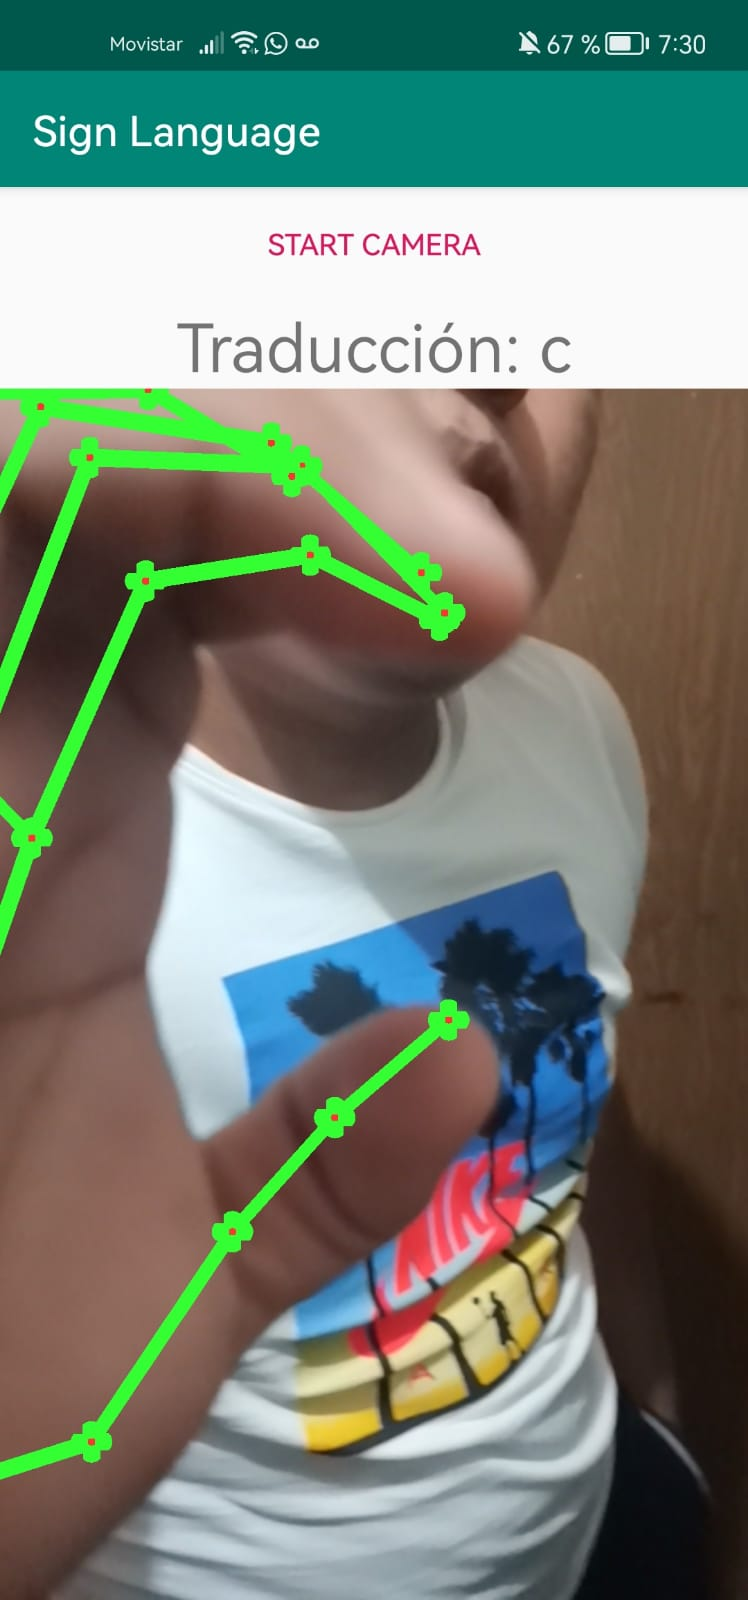
\includegraphics[width=0.16\textwidth]{2022_AplicacionLSM/figs/App1.jpeg}
    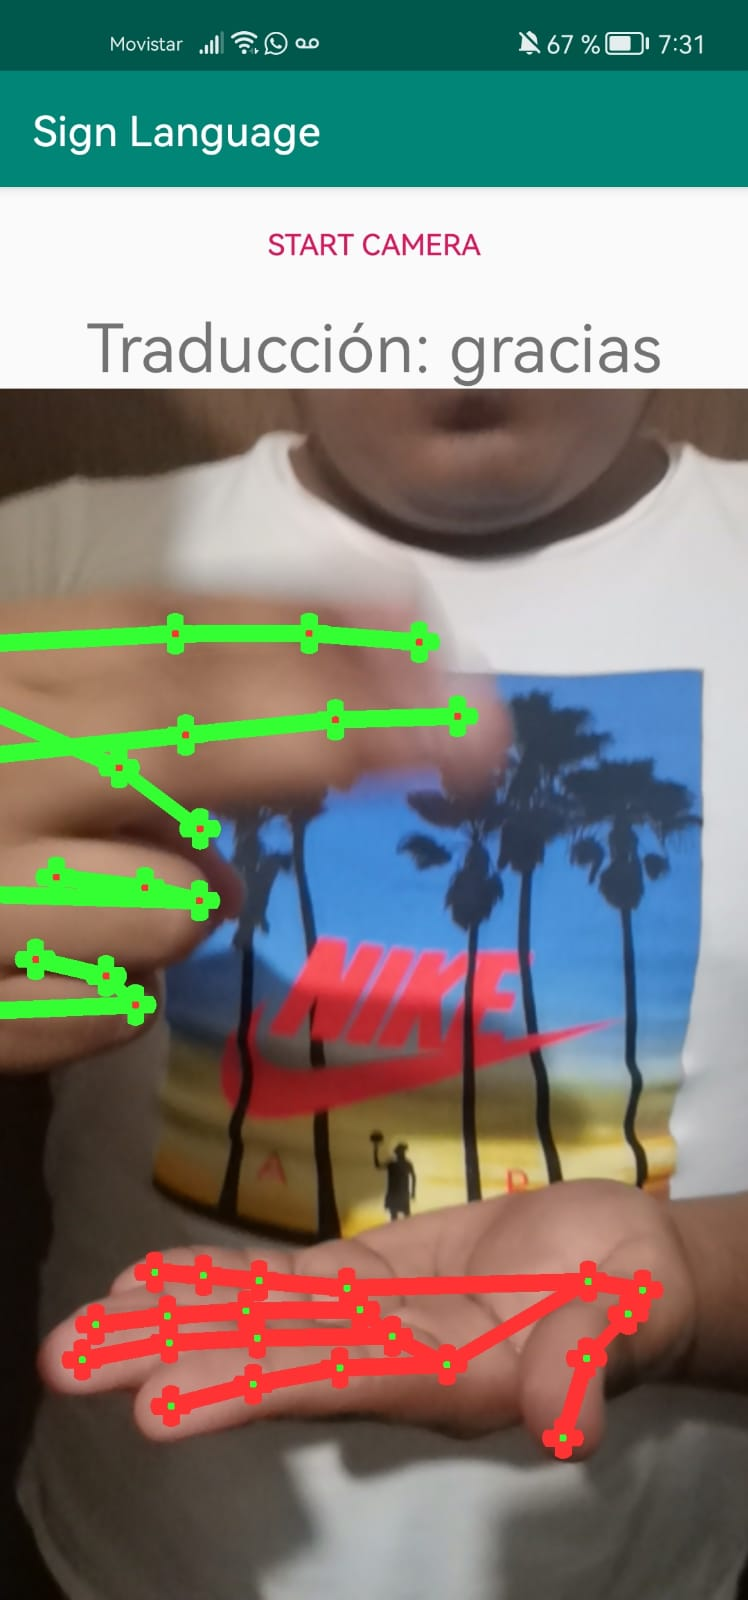
\includegraphics[width=0.16\textwidth]{2022_AplicacionLSM/figs/App2.jpeg}
    \includegraphics[width=0.16\textwidth]{2022_AplicacionLSM/figs/Muestra_compañeros1.jpeg}
    \includegraphics[width=0.16\textwidth]{2022_AplicacionLSM/figs/Muestra_compañeros2.jpeg}
  \end{tabular}
\end{center}

\end{frame}






